\documentclass[11pt]{article}
%Gummi|065|=)
\title{\textbf{DIagrama electrico de interfaz de potencia. }}
\author{Guzman Vazquez Jaime Alan Yamil.}
\date{10 de noviembre del 2019}
\usepackage{graphicx}
\begin{document}

\begin{center}
\LARGE \textbf{Universidad Politecnica de la Zona Metropoilitana de Guadalajara\\}


\begin{figure}[htp]
\centering

\includegraphics[scale=1.00]{/home/emile/Escritorio/guzman.vazquez.jaime.alan.yamil/practicas/Ev_3_1_Diagrama_electrico_de_la_interfaz_de_potencia./Upzmg9.png}
\caption{}
\label{}
\end{figure}

\large \textbf{Diagrama electrico de la interfaz de potencia}\\
\vspace{0.1cm}
\large \textbf{Nombre: \\Guzman Vazquez Jaime Alan Yamil.\\Rodriguez Lopez Francisco Javier.\\
\vspace{0.1cm} Matricula:\\18311861\\18311804.\\
\vspace{0.1cm} Carrera: Ingenieria en Mecatronica.\\
\vspace{0.1cm} Materia: Sistemas Electronicos de Interfaz.\\
\vspace{0.1cm} Curso: septiembre-diciembre del 2019.\\
\vspace{0.1cm} Docente: Moran Garabito Carlos Enrique.}


\vspace{0.5cm}
\small \textbf{10 de Noviembre del 2019}
\end{center}

\section{Introducción:}

Las interfaces de potencia, requeridas en el curso de la materia, se han estado expandiendo, a medida de practicas, tales, como la practica 8, la pratica 9 consta de ello, ver en un sistema de diagramas, el sistema de control de potencia, a partir de los acomodos, y de ello, del aprendizaje, que va obtendiendo en la generacion y realizacion de estas practicas.\\

Lo que se estara viendo, en la practica 9, es la realizacion de 3 diagrams squematicos, cada unmo cuimpliendo si funcion, en cada uno de los casos, se estara viendo, lo utilizado en la ultimaa etapa de la transformacion CD/CD, la cual se vera a partir de otros diagramas, que nos puedan ayudar, en la generacion y emejoramiento de la potencia disipada, a manera de ver los arreglos que se les puede dar a estos, y como de ellos, se puede mejorar el control que se tiene ya establecidfo, en los convertidores.\\

Conceptuando en este reporte, la realizacion de ellos, y la generacion a partir de dichas ideas, y aprendizaje generado, en las clases de pratica, generando dos de los sistemas, de un comportamiento de doblaje, o disminucion de potencia y de ello voltaje, en constancia a un arreglo, adicional, el cual se estara explicando de manera mas a fondo, en el desarollo de este reporte, y como de ello, se puede generar la dicha disminucion u doblaje de voltaje requerido, para la referencia de practicas anteriores, con un acomodo de mejor estancia y control. 


\section{Objetivo:}

Generar a partir de un campo magnetico, la disminucion o duplicacion de voltaje y corriente.

\section{Material:}

\begin{itemize}
\item Baterias de 1.5v.
\item Bobinas de 106 vueltas y 82 vueltas.
\item Capacitores (100uF a 25v, 10uF a 50 v, 220pF a 25v).
\item Diodos Led.
\item Fuente de 12v.
\item Mosfet (IRF640N).
\item Resistencias (47 ohm, 68 ohm, 220 ohm).
\item Transistor Tip41c.
\item Transistor Tip31c.
\item Transformador de pulsos o bobina con doble campo magnetico.
\end{itemize}
\newpage
\section{Procedimiento:}

Para la realizacion de esta practica, el docente, establecio tres diagramas, los cuales cada uno consistia en una tarea diferente, a partir del acomodo y generacion del calculo corresponidnete, para el sistema del campo magenitco y como esto se establece de mejor forma, en un enrollamiento de cobre, el cual genera entre mas vueltas un campo magnetico mayor, y a ello, un sistema de disminucion o duplicacion de voltaje y corriente, asi tambien como la potencia trabajada, en cada parte del sistema a trabjar, en este caso, siendo cada uno de ellos, diferente al otro, pero en reflejo de ello igual, asi que esta parte puede confundir un poco, el para que de estos acomodos, si en su observacion se reflejan iguales, y la utilizacion de los mismos, componentes, y es ahi cuando entra el acomodo que se da a cada uno de estos, ya que si por una parte el campo magnetico, se genera de una parte al princiipio este, hara que la potencia disipada, incremente el voltaje y de ello la potencia, pero sin embargo, otra parte, pueda hacer que la bobina, se encuentre despues del inicio, lo que hace que el campo magenitco generado, sea este menor o mayor, se refleje en la disminucion del voltaje y potencia requerida.Tal y como se muestra en los diagramas establecidos.\\

A)\\

\begin{figure}[htp]
\centering
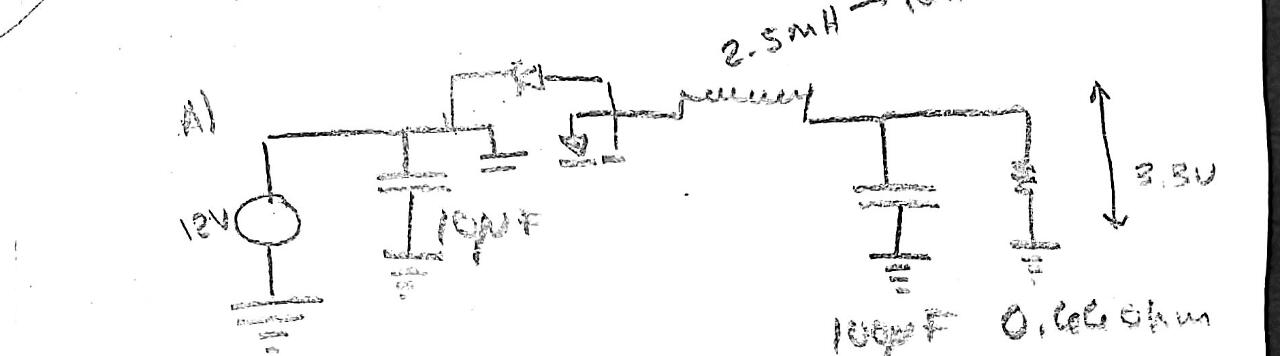
\includegraphics[scale=0.50]{/home/emile/Escritorio/guzman.vazquez.jaime.alan.yamil/practicas/Ev_3_1_Diagrama_electrico_de_la_interfaz_de_potencia./esquema1.jpeg}
\caption{}
\label{}
\end{figure}

En el primer esquematico, se tiene como control a un Mosfet, el cual nos ayuda, desde su integrado de un diodo zener, el cual rectifica de mejor forma, la entrada del voltaje de 12v, antes de ello, esta puesto un capacitor de 10uF, esto para que al momento de llegar al Mosfet, este no llegue de lleno a los 12v, sino que se deteriore un poco, desde este punto la entrada del voltaje puesto. Despues de haber colocado, el punto anterior, viene el inductor, puesto en marcha, como la parte impornate de este esquema, esta tiene que generar un camp magnetico de 2.5mH, el caul ayuda a que este circuito, sea de disminucion de voltaje, respecto a la colocacion en la que se encuetra, el inductor, y cuanto es el campo magentico que genera este, al estar excitado.\\

A ello se le coloca de salida, un condensador de mayores Faradios, ya que al ser puesto de mayor Faradio que el primero, este regula de mejor forma el volatej drecyo, haciendo mas lineal, el voltaje de salida, y en su puesta a ello, una resistencia de muy pocos ohmios, ya que si le agregaramos mas ohm, este recibiria el puesto mas grande de satiracion de boltaje y corriente, y en ello, el voltaje no disminuiria, sino que simplemente lo satiraria, es por eso que se coloca, una resistencia tan baja como lo es la de 0.66 ohm. En este caso, no se dispuso de una resistencia tan baja por lo que se contruyo una resietncia, la mas baja que se pudo realizar, quedando en puesta 4 resistencias de 68 ohm en paralelo generando una salida de saturacion de 17 ohm, respecto a esta salida, el voltaje de salida, nos da como generamiento de ello, 3.6v, lo cual al meterle de lleno los 12v, queda por hecho este circuito.
\newpage
B)\\

\begin{figure}[htp]
\centering
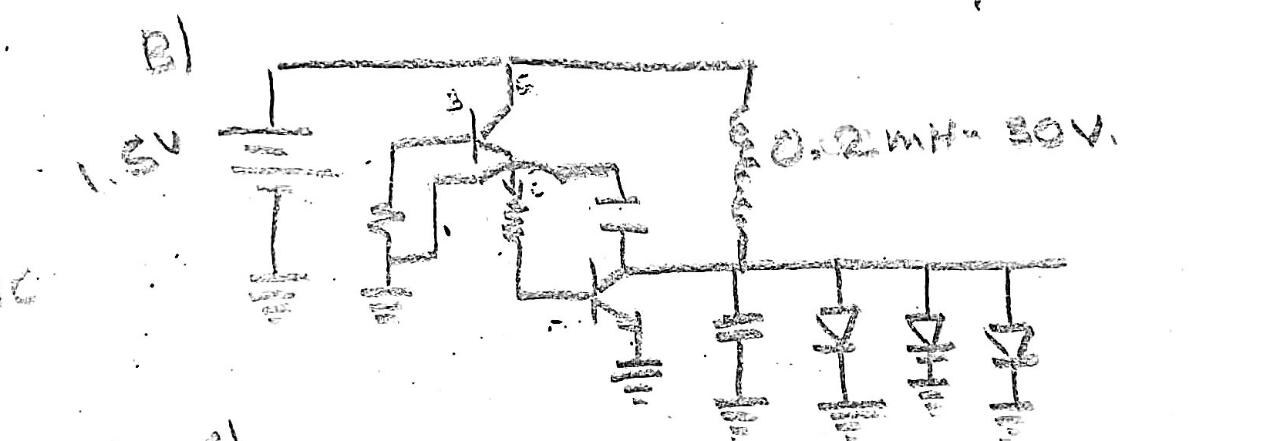
\includegraphics[scale=0.50]{/home/emile/Escritorio/guzman.vazquez.jaime.alan.yamil/practicas/Ev_3_1_Diagrama_electrico_de_la_interfaz_de_potencia./esquema2.jpeg}
\caption{}
\label{}
\end{figure}

Este diagrama, tiene como caracteristica, elevar el voltaje, ya sease al doble de su capacidad inicial, o un poco menos de eso, esto ya dependiendo, el colocamiento que se tenga en esto, en est ecaso, se tiene como entrada una bateria de 1.5v, se establecio este pequeño voltaje, para el encendido de unos leds, como prueba de su elevacion, y estancia de ello, su acomodo. En su parte positiva de la bateria, se tiene un Tip41c, se utiliza un transistor de alta potencia, ya que la generacion de ello, tiene que ser su objetivo, tener a la entrada una potencia baja, pero a la salida, una potencia mayor, y este en su acomodo, puede realizar ese trabajo, se tienen dos, ya que la potencia disipada, en el inductor es menor al del esquematico anterior, ya que este no debe de generar un campo magnetico tan grande, sino que solo tiene que inducir lo necesario, para transmitir el voltaje, este es el contrario al transistor, ya que este dobla solo la potencia, y la transimite a partir de la corriente.\\

De ello, tenemos una salida con un condensador, en esta parte se cumple la misma funcion que en el caso anterior, ya que la onda generada a partir del condensador, es lineal, convirtiendo mas pura la salida de la potencia, haciendo que los 3 leds, puestos com prueba de ello, prendan sin problemas, aunque aqui se genera una complicacion, ya que el circuito empieza  a doblar su voltaje, y potencia, cuando es colocada un voltaje de 2.6v, por lo que los 1.5 de la bateria, no son suficientes, para la conmutacion y doblamiento de la potencia requerida a la salida. Se debe de tener en cuenta, el campo magentico generado, generado por el inductor, ya que si este es muy grande, o en reversiva a ello, muy pequeño, generando complicaciones, a la salida de potencia, voltaje y corriente.\\

C)\\

\begin{figure}[htp]
\centering
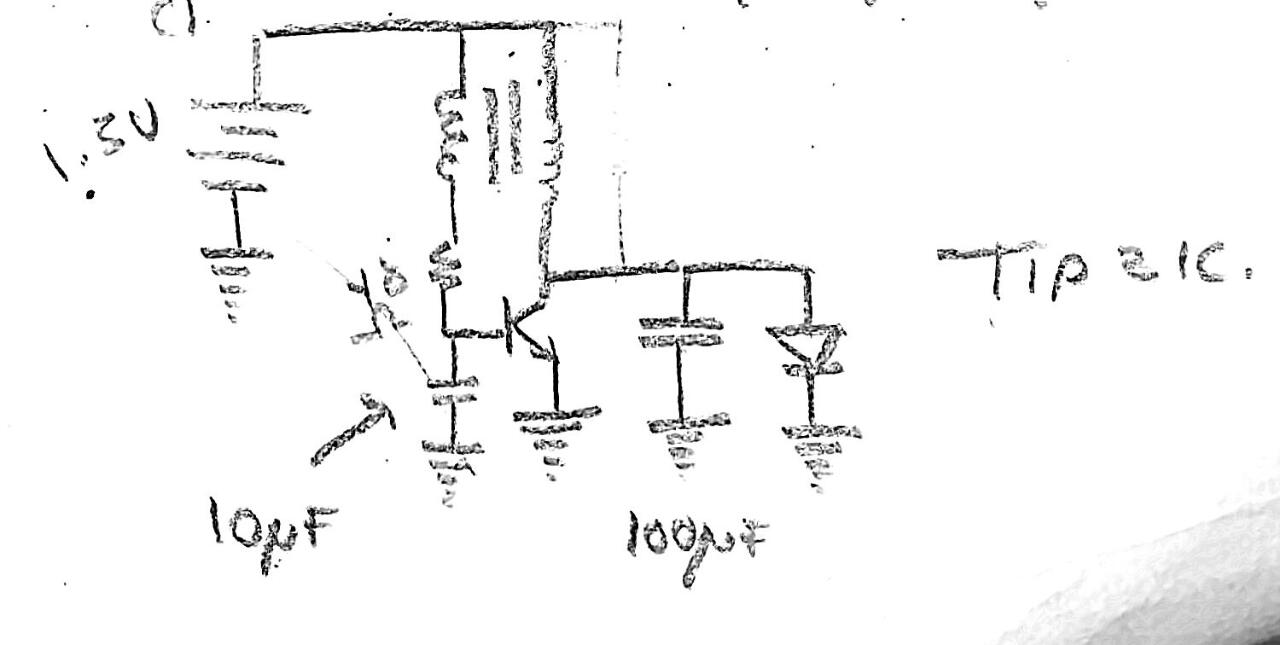
\includegraphics[scale=0.50]{/home/emile/Escritorio/guzman.vazquez.jaime.alan.yamil/practicas/Ev_3_1_Diagrama_electrico_de_la_interfaz_de_potencia./esquema3.jpeg}
\caption{}
\label{}
\end{figure}

Este ultimo circuito, tiene como objetivo elevar el voltaje, pero en este caso, se tvo complicaciones, las cuales se tuvieron en cuenta, ya que a la entrada se tiene una bateria de 1.5v, generado como en el esquematico anterior un duplicador del voltaje de inicio, en relevancia a ello, y la colocacion, que se tiene en el esquematico, en donde se encuetra un transformador, de la entrada de ellos, al positivo de la bateria, en este caso, se tuvo a la disposicion un transformador y un solenoide de doble enrollamiento, en este caso, para suplementar al transofrmador, se tiene como perpectiva, que cualquiera de los dos componentes, se comporten de la misma forma, ya que el tornillo, al tener un enrollamiento, y se pone encima de ello, otro enrrollamiento, con un calibre menor de cobre, se tiene que tener en cosntancia un transformador, ya que tiene en si, dos campos magenticos, para generar.\\

En una terminal del campo magentico 2, se coloca a ello, el conector del transistor Tip31c, ya que este transistor al igual que el anterior, es de alta potencia, al hacer esto, se espera que tambien duplique el voltaje de entrada, y por otra parte, se tiene a la terminal del campo magnetico 1, conectado a una resistencia de 220 ohm, y de ello, la conexion a la base, se coloca una resistencia en este punto, para la saturacion de voltaje disipado por el inductor, y de ello el emisor del transistor se situa en tierra, asi como en los casos anteriores, se pone un condensador a la salida de voltaje, para que esta realice lo msimo que seria, tener el voltaje de manera mas lineal, que al principio, y a ello, un diodo Led, para el señalamiento de la duplicacion de voltaje, pero en este caso, hubo al igual que en el anterior fallas, ya que en ocasion a duplicar, resta a la mitad, el voltaje que tenemos a la entrada, siendo este circuito, restador, para asi tener a la salida, un voltaje de menor potencia y menor voltaje, pero con la misma corriente de entrada, dejando ver, que la disipacion de los campos magneticos, es mucha, y de ello la disminucion de voltaje.\\

Nota: Todas las salidas van a tierra, esto para generar la comunicacion con la segunda parta de cada uno de los componentes a usar.

\section{Resultados:}

A)\\

Se tiene que generar y armar un inductor, con un campo magentico de 2.5mH, por lo que la generacion del solenoide, queda establecida por el un calculo, el cual nos deja ver las vueltas que se les tiene que dar, para la generacion de este campo magnetico. \\

Formula utilizada:\\
$$ n=\sqrt{\frac{L*Cx10^{8}}{1,256 x S}} $$

Obteniendo, los datos a partir del tornillo utilizado, queda como:\\
$$ n=\sqrt{\frac{2.5mH*0.014x10^{8}}{1,256 * 1.5x10^{-4}}}= 106 vueltas. $$

La superficie, es $ \pi $ por radio al cuadrado, por lo que la generacion de esto, se saca, a partir de datos obtenidos.\\
$$ S=\pi * r^{2} $$
\newpage
Quedando como:\\

$$ S=\pi * \frac{0.014m}{4}^{2}= 1.5x10^{-4} $$

Teniendo en cuenta las vueltas que se le daran al soneloide, este sera el sufucinete, para generar el campo magentico requerido, a partir del cobre que se tenga. Dejando una disminucion de 3.6v.\\

\begin{figure}[htp]
\centering
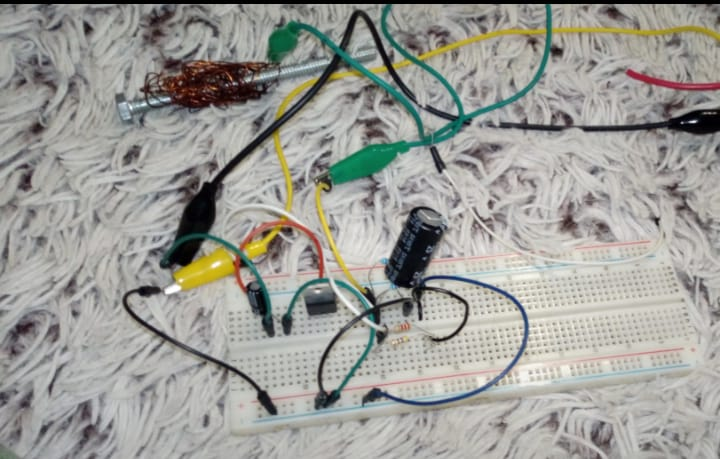
\includegraphics[scale=0.50]{/home/emile/Escritorio/guzman.vazquez.jaime.alan.yamil/practicas/Ev_3_1_Diagrama_electrico_de_la_interfaz_de_potencia./resul1.jpeg}
\caption{}
\label{}
\end{figure}

B)\\

En este caso, se establecen ya las vueltas que se tienen que dar, pero en este caso, el campo magentico generado con 30 vueltas, es muy poco, por lo que queda establecido de la siguiente forma:\\
$$ L=1,256* \frac{S * n^{2}}{C}x10^{-8} $$

Simplificando datos:\\
$$ L=1,256* \frac{1.5x10^{-4} * 30^{2}}{0.014m}x10^{-8}= 0.4mH $$

En este caso, es muy poco el campo magnetico generado, por lo que se queda establecido, que las vueltas deberian de ser mas, para un campo magentico mayor:\\
$$ n=\sqrt{\frac{1.5mH*0.014x10^{8}}{1,256 * 1.5x10^{-4}}}= 82 vueltas. $$

Generando asi el campo magnetico requerido, para la duplicacion de voltaje, y el encendido de los Led.\\

\begin{figure}[htp]
\centering
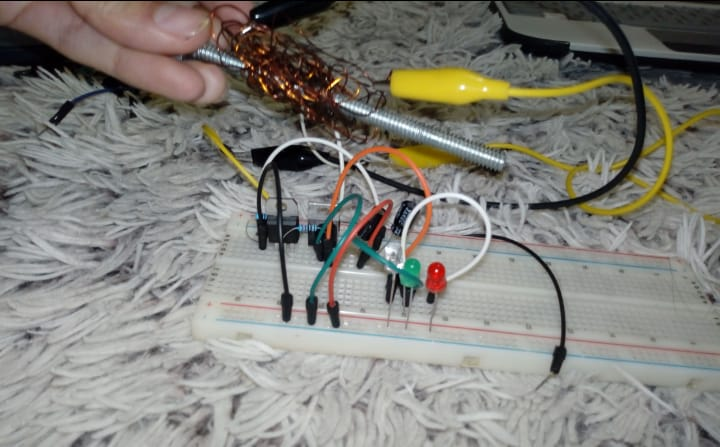
\includegraphics[scale=0.50]{/home/emile/Escritorio/guzman.vazquez.jaime.alan.yamil/practicas/Ev_3_1_Diagrama_electrico_de_la_interfaz_de_potencia./resul2.jpeg}
\caption{}
\label{}
\end{figure}

C)\\

El calculo, para este caso, es el mismo que en el caso 1, simplemente a este se le añade, doble embobinado, para asi poder tener en cuenta el transformador que se requiere, los resultados lanzados n este caso, dan por generacion un campo magnetico de 5mH, por lo que el campo magentico es mucho mayor a los dos casos anteriores, y de ello, la generacion en su relacion, con la comunicacion de los componentes y su transmision de ellos.

\begin{figure}[htp]
\centering
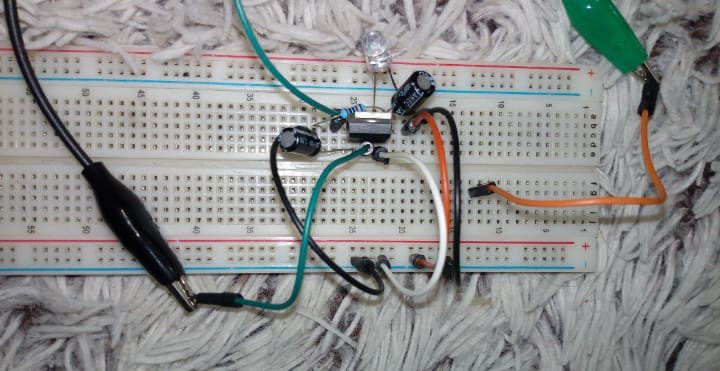
\includegraphics[scale=0.50]{/home/emile/Escritorio/guzman.vazquez.jaime.alan.yamil/practicas/Ev_3_1_Diagrama_electrico_de_la_interfaz_de_potencia./resul3.jpeg}
\caption{}
\label{}
\end{figure}

\section{Conclusión:}

CONCLUSION:Jaime Guzman.\\\

Esta aplicacion dada por estos tres circuitos es muy relevante para el mundo de la electrónica debido a que permite a dispositivos de bajo consumo o de voltaje bajo a convivir con dispositivos de voltaje alto debido a esta podría llamarse control de voltaje.\\\\
Este tipo de circuitos tienen un gran grado de libertad en cuestión de aplicaciones practicas debido a la gran variedad en el consumo de energía de los diferentes dispositivos así como las diferentes propiedades de cada uno los hacen muy útiles y versátiles para las diferentes implementaciones que se requieran en los diferentes proyectos en los que se quieran ver implementados.\\



\textbf{\Large Referencias:}\\
Carlos Enrique Móran Garabito, Sistemas Electronicos de Interfaz, Curso: Sep-Dic 2019 c, Diagrama electrico de la inertfaz de potencia.






\end{document}
